% !TeX root = ../main.tex
% !TeX encoding = UTF-8

\subsubsection{Prediction Performance across Levels of Deviation from Routine Patterns}\label{sec:scenario-performance}\label{sec:exp-scenarios}

All-grid spatial statistics describe flow distribution at a given time. To examine prediction error under deviations from routine levels, we grouped observations by window, grid cell, and channel. At positions with positive H6 target flow, RBSRN was compared with 16 baselines. Chengdu scenario analysis and the subsequent residual diagnostics use a dedicated diagnostic checkpoint, whose full-test-set H6 MAE is 0.709952 for inflow and 0.709944 for outflow. The main Chengdu tables use the comparison checkpoint. Shanghai scenario analysis and residual diagnostics use the epoch-115 checkpoint reported in the main tables.

The routine-flow reference is the median training flow for the same grid cell, channel, 5-minute slot, and weekday/weekend type. We used deduplicated training-history timestamps that passed the quality checks. If a slot had fewer than four observations for one day type, the two types were pooled; if it had none, we used the grid-cell and channel median. We divided each observation's difference from its reference by a robust scale to obtain the standardized residual \(r_k\). The scale is the training residual median absolute deviation multiplied by 1.4826, with a lower bound of 1 count. The input-window deviation score is \(D=\frac{1}{12}\sum_{k=1}^{12}|r_k|\). For each city and channel, we pooled grid cells from training windows whose 12 historical steps passed the quality checks. The 50th, 80th, and 95th percentiles of \(D\) define four groups (Table~\ref{tab:scenario-group-thresholds}); boundary values enter the lower group.

% !TeX root = ../main.tex
\begin{table}[!htbp]
  \centering\footnotesize
  \caption{Scenario-group thresholds from training data}
  \label{tab:scenario-group-thresholds}
  \setlength{\tabcolsep}{4pt}
  \begin{tabular}{llrrrrrr}
    \toprule
    City & Channel & \(D_{50}\) & \(D_{80}\) & \(D_{95}\) & \(U_{75}\) & \(B_{1/3}\) & \(B_{2/3}\) \\
    \midrule
    Chengdu & Inflow & 0.166667 & 0.583333 & 1.083333 & 1.636364 & 0.279326 & 0.453125 \\
    Chengdu & Outflow & 0.166667 & 0.625000 & 1.083333 & 1.636364 & 0.287192 & 0.471179 \\
    Shanghai & Inflow & 0.281038 & 0.708333 & 1.096048 & 1.636364 & 0.311065 & 0.489387 \\
    Shanghai & Outflow & 0.250000 & 0.674491 & 1.083333 & 1.590909 & 0.311294 & 0.492517 \\
    \bottomrule
  \end{tabular}
\end{table}


\begin{figure}[!htbp]
  \centering
  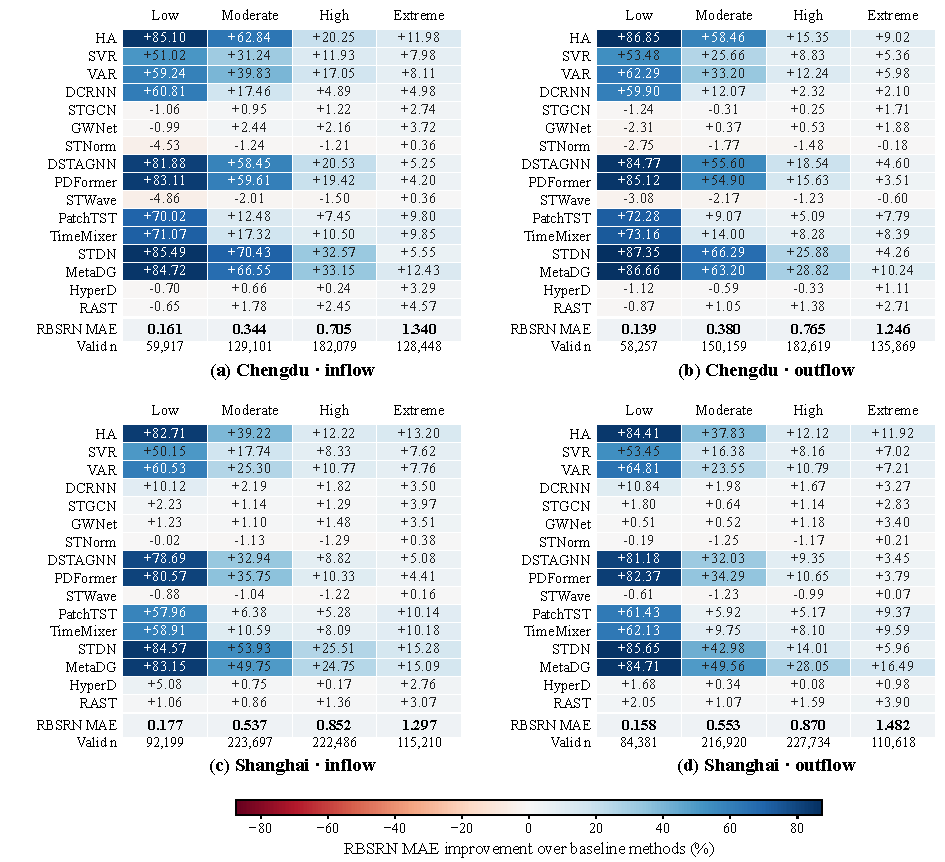
\includegraphics[width=\linewidth]{figures/scenarios/performance_h6_paper.pdf}
  \caption{RBSRN relative MAE at H6 across deviation groups.}
  \label{fig:scenario-performance}
\end{figure}

Figure~\ref{fig:scenario-performance} compares methods within each group; positive values indicate an MAE reduction relative to the corresponding baseline. In the Extreme group, RBSRN had the lowest MAE for Chengdu inflow, Shanghai inflow, and Shanghai outflow, with reductions of 0.36\%, 0.16\%, and 0.07\% relative to STWave. For Chengdu outflow, RBSRN ranked third, with MAE 0.60\% above STWave. STWave and STNorm had lower errors than RBSRN in the Moderate and High groups on all four tasks.

Absolute MAE increased with deviation level on all four tasks. Extreme-group MAE was 7.33--9.37 times the Low-group value. For Chengdu inflow, MAE increased from 0.161 to 1.340 while mean positive-target flow increased from 1.160 to 3.637 counts per 5 min, so the group differences reflect both deviation level and flow magnitude.

\subsubsection{Effects of SERR Residual Corrections across Recent-Change Scenarios}\label{sec:scenario-serr}

Within the high-deviation subset combining High and Extreme observations (\(D>D_{80}\)), recent-change intensity is defined by successive differences in historical standardized residuals:
\begin{equation}
  U=\frac{1}{11}\sum_{k=2}^{12}|r_k-r_{k-1}|.
  \label{eq:scenario-recent-change}
\end{equation}
The 75th percentile of \(U\) among high-deviation training samples separates Slow and Rapid groups; values above the threshold enter Rapid.

We examined each residual correction with a fixed-model residual-removal diagnostic. Model parameters, gates, and all other outputs were held fixed while one specified correction was subtracted from the final prediction:
\begin{equation}
  \Delta\mathrm{MAE}_{e}
  =\mathrm{MAE}(\widehat Y-C_e)-\mathrm{MAE}(\widehat Y),
  \label{eq:scenario-residual-removal}
\end{equation}
Here, \(C_e\) is the signed correction added to the prediction, including the original gating weight, learnable strength coefficient, and inverse-standardization scale. Removing the SERR self-evolution expert subtracts its weighted difference from the base prediction; removing the directed time-lagged expert subtracts its weighted correction; removing BCMS subtracts the full cross-region correction. Gating weights retain their original values and are not renormalized. A positive difference means that the correction reduced group-average MAE. Because the loss is nonlinear, differences for separate corrections are not additive. This diagnostic complements the independently retrained ablations in Section~\ref{sec:exp-ablation}: it measures sensitivity of one fixed model, whereas the ablations compare retrained configurations.

In Figure~\ref{fig:scenario-serr}, all 16 removal differences across the eight city--channel--change groups were positive. The self-evolution correction benefit in Rapid was 1.15--2.82 times the Slow-group benefit, whereas the directed time-lagged correction was smaller. Its Rapid-group benefit was higher than its Slow-group benefit in Chengdu and lower in Shanghai.

\begin{figure}[!htbp]
  \centering
  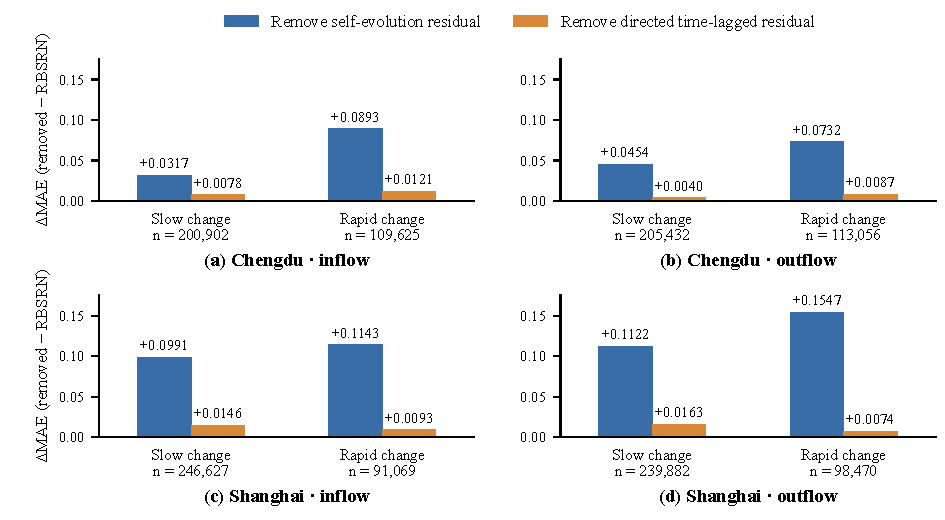
\includegraphics[width=0.92\linewidth]{figures/scenarios/serr_sensitivity_h6_paper.pdf}
\caption{H6 SERR residual-removal sensitivity by recent-change group.}
  \label{fig:scenario-serr}
\end{figure}

\subsubsection{Effects of BCMS Residual Corrections across Background Discrepancies and Forecast Horizons}\label{sec:scenario-bcms}

We measured source--target background similarity with a history-derived discrepancy proxy. Let \(\mathcal C_i\) denote the valid fixed candidate-source set for target cell \(i\), and let \(\bar r_i\) be its mean standardized residual over the 12 historical steps. For each channel, define
\begin{equation}
  B_i=\frac{1}{|\mathcal C_i|}\sum_{j\in\mathcal C_i}|\bar r_i-\bar r_j|.
  \label{eq:scenario-background-difference}
\end{equation}
The candidate set follows the model's fixed support. \(B_i\) describes discrepancy in the observed history and is separate from the low-frequency representation learned by BCMS. Tertile thresholds estimated from high-deviation training samples define Low, Medium, and High discrepancy groups (Table~\ref{tab:scenario-group-thresholds}). We removed the full BCMS correction at H1--H12 using Eq.~\eqref{eq:scenario-residual-removal}. Both figures report MAE changes in \(10^{-3}\) counts per 5 min; each cell is \(1000\times\Delta\mathrm{MAE}\).

Figure~\ref{fig:scenario-bcms} shows a consistent ordering across city, channel, and horizon: the mean benefit was largest in the Low group, followed by Medium and High. Of 144 background-group--horizon cells, 143 were positive; the only negative value was approximately \(-4.8\times10^{-6}\) for Chengdu outflow in the High group at H5. Benefits varied across horizons without a monotonic trend.

\begin{figure}[!htbp]
  \centering
  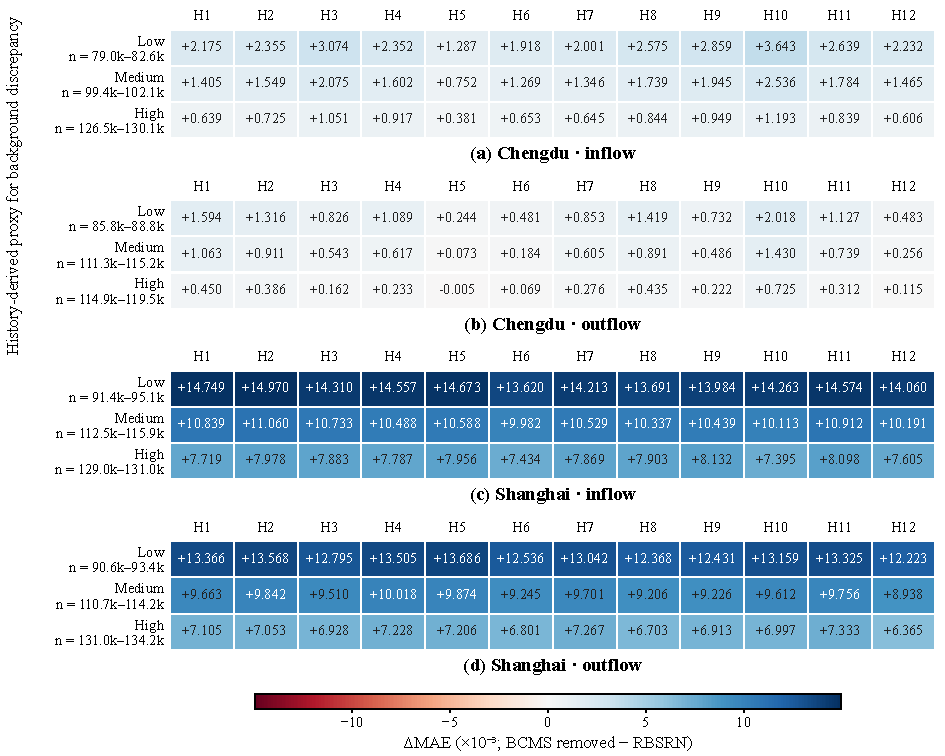
\includegraphics[width=0.92\linewidth]{figures/scenarios/bcms_sensitivity_horizons_paper.pdf}
\caption{BCMS residual-removal sensitivity in high-deviation scenarios.}
  \label{fig:scenario-bcms}
\end{figure}

Figure~\ref{fig:scenario-bcms-all} extends the analysis to the full test set with the same thresholds fitted from high-deviation training histories. All 144 removal differences were positive and exceeded the corresponding high-deviation values. The Low--Medium--High ordering persisted. For Shanghai inflow at H6, full-test differences were 0.025547, 0.015634, and 0.009873, compared with 0.013620, 0.009982, and 0.007434 in the high-deviation subset. The full-test analysis therefore shows that the average BCMS benefit extends beyond high-deviation samples.

\begin{figure}[!htbp]
  \centering
  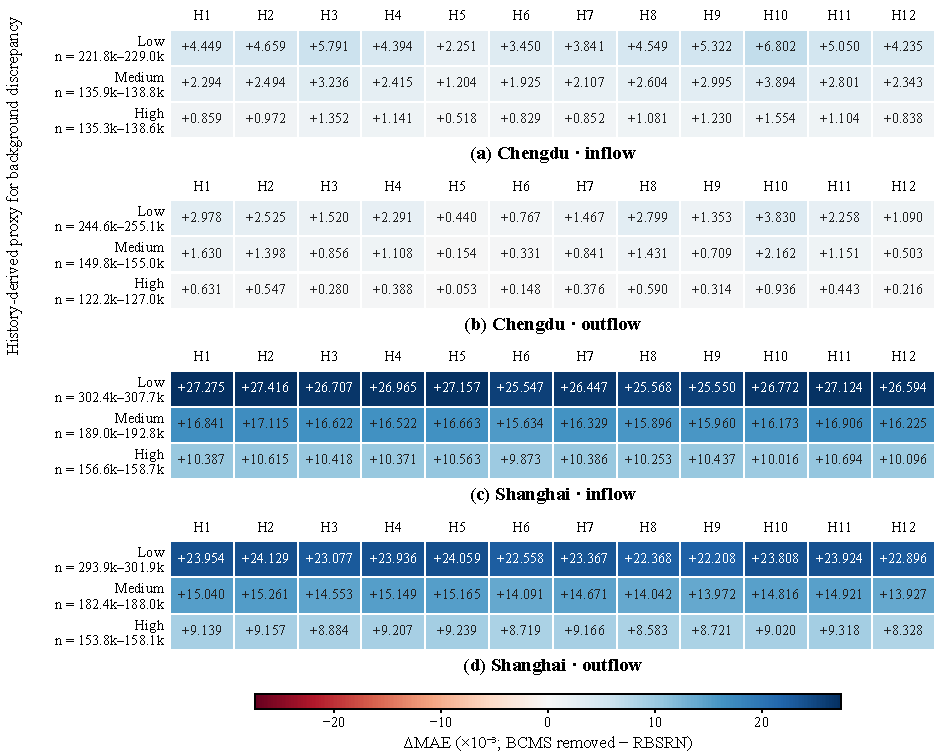
\includegraphics[width=0.92\linewidth]{figures/scenarios/bcms_sensitivity_horizons_all_test_paper.pdf}
\caption{BCMS residual-removal sensitivity across the full test set.}
  \label{fig:scenario-bcms-all}
\end{figure}
